\section{Fenómenos de transporte}
\subsection{Ley de Newton de la viscosidad}
Consideremos un fluido (líquido o gas) contenido
entre dos grandes laminas planas y paralelas, de área $A$,
separadas entre sí por una distancia muy pequeña $Y$
Supongamos que el sistema está inicialmente en reposo, pero
que al a cabo del tiempo $t=0$, la lamina inferior se pone
en movimiento en la dirección del eje $x$, con una velocidad
constante $V$, A medida que transcurre el tiempo el fluido
gana cantidad de movimiento, y, finalmente se establece
la velocidad en régimen estacionario. Una vez alcanzado
dicho estado estacionario de movimiento, es preciso aplicar
una fuerza constante $F$ para conservar el movimiento laminar
inferior. ESta fuerza viene dada por la siguiente expresión
(suponiendo que el flujo es laminar):

\begin{equation}
    \label{eq:newton:viscosity}
    \frac{F}{A} = \mu \frac{V}{Y}
\end{equation}

Es decir, que la fuerza por unidad de área es proporcional
a la disminución de velocidad con distancia $Y$. La constante
de proporcionalidad $\mu$ se denomina viscosidad del fluido.

\begin{figure}[ht]
    \begin{center}
        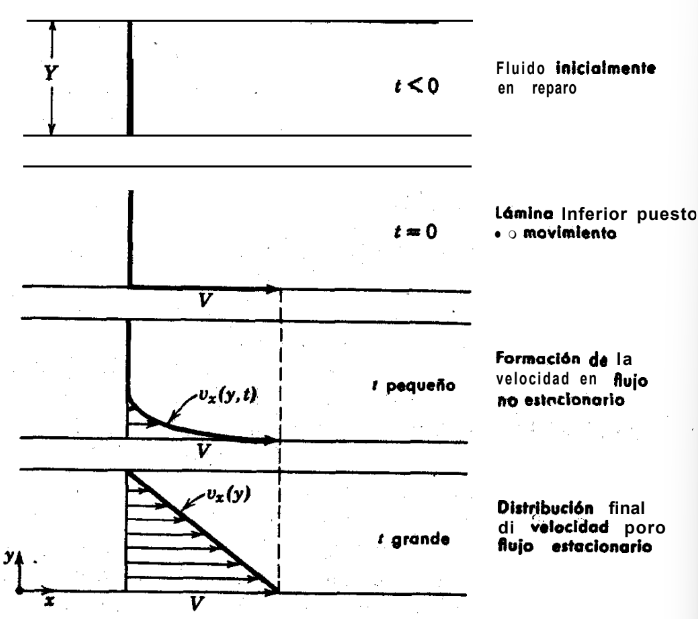
\includegraphics[scale=0.8]{sections/img/vicosidad.png}
    \end{center}
    \caption{flujo de un fluido viscoso}
\end{figure}

Si queremos utilizar la ecuación~\ref{eq:newton:viscosity}
es conveniente expresarla en una forma más explícita. El
esfuerzo constante que se ejerce en la dirección $x$ sobre
la superficie de un fluido, situada a una distancia constante
$y$, por el fluido existe en la región donde $y$ es menor,
se designa por $\tau_{xy}$ y el componente $x$ del vector
de velocidad de fluido, por $v_{x}$, Téngase en cuanta que
$v_x$ no es igual a $\partial v/ \partial x$; asi la ecuación
~\ref{eq:newton:viscosity} queda de la siguiente forma
\begin{equation}
    \label{eq:newton:explicite}
    \tau_{xy}=-\mu \frac{dv_x}{dy}
\end{equation}
Esta es la ley de \textit{Newton de la Viscosidad}
y los fluidos que cumplen se denominan
\textit{fluidos newtonianos}. Todos
los gases y la mayor parte de los líquidos sencillos,
se comportan de acuerdo a la ecuación~\ref{eq:newton:explicite}

\subsection{Ley de Poiseuille}
Consideremos un tubo de longitud $l$ y radio $R$, por cuyo interior
circula un fluido viscoso en régimen laminar; las capas de fluido
circularán en su interior con distintas velocidades,
siendo nula la velocidad de la que se encuentra en contacto con él,
puesto que queda adherida a la pared; ésta a su vez «tira» hacia atrás
de la capa más próxima a ella y así sucesivamente; la velocidad será
máxima en el centro del tubo.

\begin{figure}[ht]
    \begin{center}
        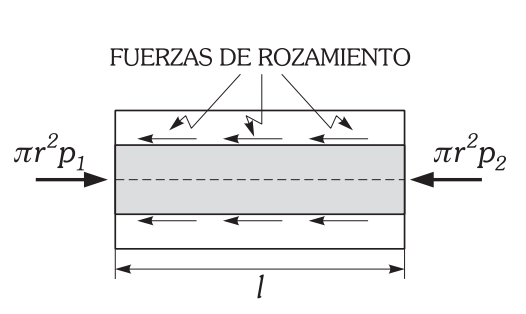
\includegraphics[scale=0.5]{sections/img/ley_de_poiseuille.png}
        \caption{Tubo de corriente que se mueve a velocidad
        constante y por tanto se encuentra en equilibrio}
    \end{center}
    
\end{figure}

Si tomamos un pequeño cilindro de radio $r$, concéntrico en el tubo
que se mueve a velocidad constante y por tanto se encuentra en
equilibrio de fuerzas; la fuerza motora debida a la diferencia de
presión entre sus extremos tendrá que igualarse a la fuerza retardadora
de viscosidad que actúa sobre su superficie lateral, y por tanto:

\begin{equation*}
    \left(p_1 - p_2\right)\pi r^2 = -\mu A \frac{dv}{dr} 
    = - \mu 2 \pi r l \frac{dv}{dr}
\end{equation*}

siendo $dv/dr$ el gradiente de velocidad de una distancia $r$
del eje, y ponemos el signo menos para indicar que la velocidad
disminuye a medida que $r$ aumenta; agrupando términos se obtiene:

\begin{equation*}
    -dv=\frac{p_1 - p_2}{2 \pi l}r dr \Rightarrow
    -\int_v^0dv = \frac{p_1-p_2}{2\mu l}\int_0^R rdr \Rightarrow
    v = \frac{p_1 - p_2}{4\mu l}\left(R^2 - r^2\right)
\end{equation*}

la ecuación $v=f(r)$ es la de una parábola y decimos que el flujo
tiene un \textit{perfil} de \textit{velocidades}
parabólico.

\begin{figure}[ht]
    \begin{center}
        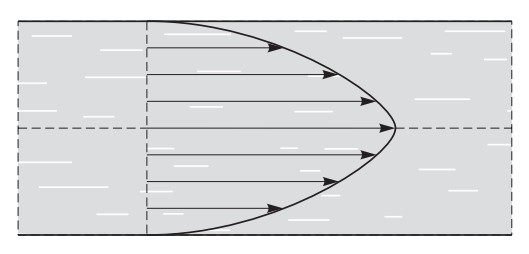
\includegraphics[scale=0.5]{sections/img/ley_de_poiseuille_parabola.png}
    \end{center}
    \caption{Perfil de velocidades parabólico}
\end{figure}

Para hallar el caudal calculemos el volumen $d^2 V$ del fluido
que atraviesa el elemento de sección recta comprendido
entre las circunferencias de radio $r$ y $r + dr$ en un tiempo
$d$, que valdrá

\begin{equation*}
    d^2V = dA v dt = 2\pi r dr \frac{p_1 - p_2}{4 \mu l}(R^2 - r^2)dt
\end{equation*}
el volumen que fluye a través de toda la sección en un tiempo
$dt$ se obtiene integrando entre $r=0$
y $r=R$ y nos queda

\begin{equation*}
    dV = \frac{\pi (p_1 - p_2)}{2\mu l}dt \int_0^R r(R^2 - r^2)dr
    = \frac{\pi R^4}{8\mu}\frac{p_1 -  p_2}{l}dt
\end{equation*}

dividiendo por $dt$ y mando $\Delta p = p_1 - p_2$,
se obtiene para el gasto $G$ la siguiente ecuación

\begin{equation}
    \label{eq:Poiseuille}
    G = \frac{\pi R^4}{8 \mu} \frac{\Delta p}{l}
\end{equation}

Que es la ecuación de Poiseuille:
El caudal de fluido (volumen por unidad de tiempo) que circula
por un tubo cilíndrico en régimen laminar, es directamente
proporcional a la cuarta potencia del radio $R$ y a la diferencia
de presiones entre la parte anterior y posterior del tubo $\Delta p$,
e inversamente proporcional a la longitud de éste $l$ y 
al coeficiente de viscosidad del líquido $\mu$

\subsection{Ley de Fourier}
La transferencia de calor $dQ$ a traves de una
barilla conductora en un tiempo determinado $dt$ es directamente proporcional a la longitud $L$ y sección transversal
$A$ de la varilla, multiplicado por $\Delta T = T_B - T_A$, donde
$T_A$ y $T_B$ son las temperaturas de los extremos de la barilla,
ademas que esta depende de la conductividad térmica $k$ del 
material, i.e.

\begin{figure}[ht]
    \begin{center}
        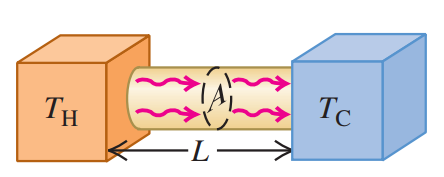
\includegraphics[scale=0.5]{sections/img/coduccion.png}
    \end{center}
    \caption{Conducción del calor }
\end{figure}

\begin{equation*}
    \label{eq:conduccion}
    H = \frac{dQ}{dt} = kAL\frac{T_A - T_B}{L}
\end{equation*}

si la temperatura varia
de manera no uniforme a traves 
de la varilla podemos
asignar la coordenada $x$ así introduciendo
la gradiente de $dT/dx$ temperatura se tiene:

\begin{equation*}
    \label{eq:conduccion-x}
    H = \frac{dQ}{dt} = \frac{-kA}{L}\frac{dT}{dx}
\end{equation*}

Ademas podemos asignar $R = L/(kA)$, siendo $R$ la resistividad
térmica, con lo que la ecuación quedará

\begin{equation}
    \label{eq:conduccion-r}
    H = \frac{dQ}{dt} = -\frac{1}{R}\frac{dT}{dx}
\end{equation}

Esta ley se puede puede aplicar a gases, sólidos y líquidos,
siempre que el transporte de calor se produzca únicamente
por conducción.

\subsection{Convección}
La convección es transferencia de calor por movimiento de una masa de fluido de una
región del espacio a otra.

La transferencia de calor por convección es un proceso muy complejo, y no puede
describirse con una ecuación sencilla. Veamos algunos hechos experimentales:

\begin{enumerate}
    \item  La corriente de calor causada por convección es directamente proporcional al
    área superficial. Esto explica las áreas superficiales grandes de los radiadores y
    las aletas de enfriamiento.

    \item La viscosidad de los fluidos frena la convección natural cerca de una superficie
    estacionaria, formando una película superficial que, en una superficie vertical,
    suele tener el mismo valor aislante que tiene 1.3 cm de madera terciada (valor
    R = 0.7). La convección forzada reduce el espesor de esta película, aumentando
    la tasa de transferencia de calor. Esto explica el “factor de congelación”: nos
    enfriamos más rápidamente en un viento frío que en aire tranquilo a la misma
    temperatura.

    \item a corriente de calor causada por convección es aproximadamente proporcional 5/4 
    nal a la potencia de la diferencia de temperatura entre la superficie y el cuerpo
    principal del fluido.

\end{enumerate}

De estas observaciones se puede en un principio 
    deducir la ley de enfriamiento de Newton

\begin{equation}
    \label{eq:enfriamiento-newton}
    q = hA(T_w - T_\infty)
\end{equation}
donde $q$ es la rapidez de transferencia del calor,
que esta relacionado directamente proporcional a $h$ llamado
el coeficiente de transferencia por convección y $A$ el área
de la superficie de contacto entre el fluido y la superficiales,
ademas $T_w$ es la temperatura de la superficie y $T_\infty$,
la temperatura suficientemente lejos de la superficie.

\subsection{Radiación}
La radiación es la transferencia de calor por ondas electromagnéticas como la luz visible,
los rayos infrarrojos y la radiación ultravioleta. Todos hemos sentido el calor de
la radiación solar y el intenso calor de un asador de carbón o las brasas de una chimenea.
Casi todo el calor de estos cuerpos tan calientes no nos llega por conducción ni
por convección en el aire intermedio, sino por radiación. Habría esta transferencia de
calor aunque solo hubiera vacío entre nosotros y la fuente de calor.

La tasa de radiación de energía de una superficie es proporcional a su área superficial A, y a T, la cuarta potencia de la temperatura absoluta (Kelvin). La tasa también
depende de la naturaleza de la superficie; esta dependencia se describe con una cantidad $e$ llamada emisividad: un número adimensional entre 0 y 1 que representa la
relación entre la tasa de radiación de una superficie dada y la de un área igual de una superficie radiante ideal a la misma temperatura. La emisividad también depende un poco
de la temperatura. Así, la corriente de calor $H = dQ/dt$ debida a radiación de un área
superficial $A$ con emisividad $e$ a la temperatura absoluta T se puede expresar como

\begin{equation}
    H = Ae\sigma T^4
\end{equation}

donde $\sigma$ es la constante de Stefan-Boltzmann.
y el valor numérico es
\begin{equation*}
    \sigma = 5.6704001402 \times 10^-8 W/m^2\cdot K^4 
\end{equation*}

\subsection{transferencia de masa}
Cuando un sistema contiene dos o más componentes cuya concentración
varía de un punto a otro, existe una tendencia natural a que la masa
se transfiera, minimizando cualquier diferencia de concentración
dentro del sistema. La transferencia de masa en un sistema se rige
por la primera ley de Fick: El flujo de difusión de una concentración
más alta a una concentración más baja es proporcional al gradiente
de la concentración de la sustancia y la difusividad de la sustancia
en el medio. La transferencia de masa puede tener lugar debido a
diferentes fuerzas motrices

\begin{figure}[ht]
    \begin{center}
        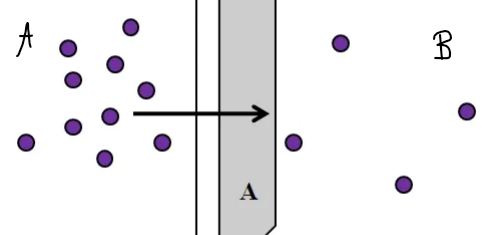
\includegraphics[scale=0.5]{sections/img/masa.png}
    \end{center}
    \caption{Moléculas transportándose de mayor concentración
    a menor concentración}
\end{figure}

\subsubsection{Difusión}
La difusión está caracterizada por el flujo
de difusión $J$ de un componente, esto es, por la
cantidad de materia que pasa en la unidad
de tiempo a través de una superficie dada en la dirección
normal a la superficie.
La densidad de flujo de difusión $j$
se puede definir como la cantidad de sustancia que
pasa en la unidad de tiempo a través de la unidad de área $S$
de la superficie dada en dirección normal a esta superficie.
asi se tiene

\begin{equation}
    \label{eq:densidad:flujo}
    j = \frac{dJ}{dS}
\end{equation}

por lo que tenemos que
\begin{equation}
    J = \int_S jDs
\end{equation}

si $j$ es constante entonces $J$ será
\begin{equation}
    J = jS
\end{equation}

\subsubsection{Fundamentemos de la difusión Molecular}
\begin{enumerate}
    \item Difusión es el mecanismo por e cual se produce el movimiento,
    debido a un estimulo físico, de un componente a través de una 
    mezcla.

    \item La principal causa de la difusión es la existencia de un gradiente de 
    concentración del componente que difunde. El gradiente de concentración provoca
    el movimiento del componente de una dirección tal que tiene a igualar las concentraciones y reducir el gradiente.
\end{enumerate}

\subsubsection{Difusión Molecular}
\begin{enumerate}
    \item Se produce por el movimiento de las moléculas individuales, debido a su energía térmica.
    \item El número de colisiones entre partículas es mayor en la zona de alta concentración, por lo que se da un flujo hacia la de menor concentración.
\end{enumerate}

\subsubsection{sistema para el estudio de la difusión molecular}
En el sistema a considerar es la película gaseosa comprendida entre la superficie del líquido y la boca
del tubo. En película gaseosa, muy cerca a la superficie líquida, se puede tomar la concentración de la especie, 
A como la de equilibrio como el líquido, es decir, 
que es la relación entre la presión de vapor de A
a la temperatura del sistema y la presión total, suponiendo
que $A$ y $B$ forman una mezcla gaseosa ideal,
dentro dle recipiente el soluto $A$ difunde a través de $B$ estancado.

\subsubsection{Ley de Fick}
La densidad de flujo de difusión es un vector. Considerando que
el valor de una de sus componentes es positivo cuando ésta esté dirigida
hacia el sentido positivo del eje, y negativo en caso contrario.

Como la sustancia se traslada de los lugares de mayor concentración a los
de menor concentración, el signo de la componente del flujo en una dirección
será el contrario del que da la derivada de la concentración en esa
dirección $(\partial c/ \partial n)$. Si la concentración 
aumenta de izquierda a derecha, el flujo va hacia la izquierda y viceversa.
Además, si la concentración de la solución es uniforme $\partial c / \partial n = 0$,
no habrá flujo de difusión. Considerando todo esto, para
un sistema estacionario macroscópico de dos componentes, homogéneo en lo que
respecta la temperatura y presión, la densidad
de flujo de difusión de uno de los componentes, debido a difusión molecular, 
vide dada por la \textit{Ley de Fick}

\begin{equation}
    j_i = -D \frac{\partial c_i}{\partial n}
\end{equation}

o utilizando la gradiente

\begin{equation}
    \vec \jmath = -D \vec \nabla c_i
\end{equation}


\begin{equation}
    J_A = D_{AB} \frac{-dC_A}{dz}
\end{equation}

donde $c_i$ es la concentración local de la sustancia, puede
medirse en masa por unidad de volumen, moles por unidad de volumen, etc.

\subsubsection{Difusión molecular en Estado estacionario}

De la ley de Fick se deduce la siguiente ecuación

\begin{equation}
    N_A = (N_A + N_B) \frac{C_A}{C_T} - D_{AB} \frac{dC_A}{dz}
\end{equation}

El primer sumando es lo que se mueve de $A$ debido al flujo global
del sistema.
El segundo sumando es la densidad de flujo que resulta
de la difusión.


\begin{itemize}
    \item $D_{AB}$: difusividad del compuesto $A$ en $B$
    \item $dC_A/dz$: Gradiente de concentración del compuesto $A$ en
    la dirección de $z$.
    \item $N_A$ es la densidad de flujo del compuesto $A$ con respecto a los ejes fijos.
    \item $N_B$: densidad de flujo dle compuesto $B$ con respecto a ejes fijos.
    \item $C_A$: Concentración molar del compuesto $A$
    \item $C_T$: Concentración molar total
\end{itemize}

\subsubsection{Difusividad}
\begin{itemize}
    \item Propiedad de transporte en función de la temperatura, presión
    y la naturaleza de los componentes
    \item Se carece de datos de difusividad para 
    la mayor parte de las mezclas que tienen interés en ingeniería.
    Es preciso estimarlas a partir de correlaciones.
\end{itemize}